\chapter{Training}

\section{Loading the preprocessed data}

After processing the document into a standard and consistent from as discussed in chapter \ref{text_normalization}. the normalized form data can be stored in any database for frequently accessing the data for training purpose. In this experiment, the database used is Elastic Search. The author initially trained the classification model with only one feature ``Product name'' and the target being the lowest level of category.
Table \ref{table:AfterNormal} displays the difference in the number of records after removing the duplicate records on the normalized text. An Index in elastic search is a logical namespace for storing data in JSON format. The indexer names ``english-taxonomy-all'' contains the data before normalization. ``english-taxonomy-normal'' contains the data after normalization and removing the duplicate entries.

\begin{table}[h]
    \centering
    \caption{Record count before and after normalization}
    \label{table:AfterNormal}
    \begin{tabular}{ lll }
          \toprule
          
          \textbf{Index}& \textbf{Features} & \textbf{Count}\\
          \midrule
          english-taxonomy-all&Product name, Category & 22160\\
          english-taxonomy-normal&Product name, Category & 1507\\
          
          \bottomrule
          \end{tabular}
\end{table}

Pandas data frame \parencite{mckinney-proc-scipy-2010} provides the \textit{drop\_duplicates()} method to remove duplicate entries in the document. Code snippet in listing \ref{code:nt} has two methods ``normalize'' and ``clean''. In Pandas \parencite{mckinney-proc-scipy-2010}, ``apply'' method executes a function along a specified axis of data frame. Here for every text in the document of data frame variable ``df\_eng'', the method ``normalize'' is called to process the data. ``normalize'' function excepts a ``document'' as a parameter.  These texts are processed to remove any html tags using Beautiful Soup a python library. Using regular expression library the digits in between the characters are removed, white spaces are removed. Any special character within the text has been transformed to its normal form.

\begin{lstlisting}[language=Python,caption={Function to normalize text and remove duplicate},label={code:nt}]
    def clean(self):

        self.df_eng["name"]	= self.df_eng["name"].str.lower().apply(lambda n:self.normalize(n)) 
        self.df_eng["category"]	= self.df_eng["category"].str.lower().apply(lambda c:self.normalize(c))
        self.df_eng=self.df_eng.drop_duplicates()
       
    
    def normalize(self,doc):

        # Remove html tags 
        if doc:
            soup = BeautifulSoup(doc, 'html.parser')
            text =soup.get_text()
            text = (re.sub('[-\W]+', ' ', text))
            text = (re.sub('(?<=\d) (?=\d)', '', text))
            text = (re.sub("([a-z]\d+)|(\d+)", '', text))
            
            
            return ''.join(
            c for c in unicodedata.normalize('NFD', text)
            if unicodedata.category(c) != 'Mn')
      
\end{lstlisting}

\section{Fetch normalized data}
The normalized document is indexed in Elastic search analytic tool. In Elastic Search, the ``search'' function allows querying and retrieving data from indexed document. Code snippet in listing \ref{code:fndfes} fetches the indexed document. 

\begin{lstlisting}[language=Python,caption={Fetch normalized data from Elastic search},label={code:fndfes}]
    def getNormal(self):
        self.df_en = pd.DataFrame(columns=['name','category'])
        resp=self.es.search("english-taxonomy-normal",{"_source":["name","category"],                                  'size' : 5000,
        "query": {"match_all": {}}})
        for hit in resp['hits']['hits']:
                list_row_en = dict (name=None,category=None)            
                list_row_en["name"]=hit['_source']['name']             
                list_row_en["category"]=hit['_source']['category']
                new_row = pd.Series(list_row_en)
                self.df_en=pd.concat([self.df_en, new_row.to_frame().T], ignore_index=True)
        
        return self.df_en
      
\end{lstlisting}
\section{Train class initialization}
As illustrated in code listing \ref{code:ootc}, the class Train is instantiated by passing the normalized form of data. This is the data that will be used for training the machine learning model.
\begin{lstlisting}[language=Python,caption={Object of the Train class},label={code:ootc}]
    df_en = df.getNormal()
    train = Train(df_en)
\end{lstlisting}

The code snippet listing \ref{code:tcc} shows the initialization for attributes.
\begin{lstlisting}[language=Python,caption={Train class constructor},label={code:tcc}]
from sklearn.feature_extraction.text import CountVectorizer
class Train():
    def __init__(self,df_en):
        self.vectorizer = CountVectorizer(1,1)
        self.df_en = df_en
        self.df_category = self.df_en.groupby("category")
        self.all_category = list(self.df_category.groups.keys())
        self.vectorizer.fit(doc=df_en["name"])
        self.inputSize=len(self.vectorizer.vocabulary_)
        self.n_categories=len(self.all_category)
        self.n_hidden = 128*3
        self.rnn= RNN(self.inputSize, self.n_hidden, self.n_categorie)
        self.learning_rate=0.005
        self.criterion = nn.NLLLoss()
        self.current_loss = 0
        self.all_losses = []
\end{lstlisting}

\begin{enumerate}
    \item self.vectorizer : Is an instance of \textbf{CountVectorizer} from scikit-learn \parencite{sklearn_api}. The details of Count vectorization is in section \ref {ch_countvector}.  The argument (1,1) indicates that the vectorizer will consider individual words as the vocabulary.
    \item self.df\_category: Stores the categorical classification of input data df\_en
    \item self.all\_category : This attribute is created to store all unique categories found in the category column of the input df\_en.
    \item self.vectorizer.fit(doc=df\_en[``name"]): The fit method of the vectorizer is called on ``name'' column of input data ``df\_en'' to build the vocabulary and transform text data in to numerical representation.
    \item self.inputSize : It sets the input size of the neural network to the size of the vocabulary.
    \item self.rnn: \acl{RNN} is initialized with updated input size, and number of hidden units and the number of unique categories as the output size.
    \item self.criterion: An instance of \acf{NLLLoss} pytorch function is stored. The function to minimize or maximize is called the objective function, or criterion \parencite[Section 4.3]{Goodfellow-et-al-2016}.
    \item self.all\_losses and self.current\_loss: These attributes are used to track the loss values during the training process.
\end{enumerate}

\section{Generating random training examples}

The code listing \ref{code:rtcc} defines a method ``randomTrainingExample''. This method is responsible for generating training examples that will be used during the training process of the neural network.

\begin{lstlisting}[language=Python,caption={Train class constructor},label={code:rtcc}]
def randomTrainingExample(self):
    
    randcategory = random.choice(self.all_category)
    # get feature name from the category
    random_feature_indices = self.df_category.indices[randcategory]
    
    index = random_feature_indices[random.randint(0, len(random_feature_indices) - 1)]

    name =self.df_en.iloc[index]["name"]
    
    category_tensor = torch.tensor([self.all_category.index(randcategory)], dtype=torch.long)
    
    name_tensor = self.helper.nameToTensor(name)
    
    return randcategory, name, category_tensor, name_tensor
\end{lstlisting}

\begin{enumerate}
    \item randcategory = random.choice(self.all\_category) : This fetches random category from the list of categories extracted during the initialization of ``Train'' class  
    \item random\_feature\_indices = self.df\_category.indices[randcategory]: The indices of the randomly obtained category from step 1 is stored from the grouped dataframe ```df\_category'''
    \item index = random\_feature\_indices[random.randint(0, len(random\_feature\_indices) - 1)] :\\ Random index is obtained from the list of indices of data sample belonging to the selected category.
    \item name = self.df\_en.iloc[index]["name"]:\\ Name of the product is accessed from the ``name'' column of the data frame. It is accessed using randomly chosen index. It accesses the name (text data) associated with selected category.
    \item category\_tensor = torch.tensor([self.all\_category.index(randcategory)], dtype=torch.long : \\ A tensor is created to represent the index of the randomly selected category. This tensor will be used during training as the target label for the corresponding input "name\_tensor".
    \item name\_tensor = self.helper.nameToTensor(name): The product name is converted into a tensor with a custom defined ``helper'' class. Code listing \ref{productnametotensor} is defined within the helper class.
    

\end{enumerate}


\section{\acl{NLLLoss}}

The negative log likelihood loss is useful to train a classification problem with ``C'' classes or target labels \parencite{Paszke.03122019}. These labels are integers representing class indices. The \acl{NLLLoss} is often used with LogSfotmax activation function. In the final layer of the neural network, adding the 
$LogSoftMax$ functions return the predicted log-probabilities. The loss is calculated by comparing the predicted log probabilities with the true target labels. 






\begin{lstlisting}[language=Python,caption={Train function},label={code:train_function}]
    
def train(self,category_tensor, name_tensor):
    
    hidden = self.rnn.initHidden()

    self.rnn.zero_grad()
    # for i in range(name_tensor.size()[0]):     

    #     output, hidden = self.rnn(name_tensor[i], hidden)

    output, hidden = self.rnn(name_tensor, hidden)
    loss = self.criterion(output, category_tensor)
    loss.backward()
   
    # Add parameters' gradients to their values, multiplied by learning rate
    for p in self.rnn.parameters():
        p.data.add_(p.grad.data, alpha=-self.learning_rate)


    return output, loss.item()
\end{lstlisting}

In code listing \ref{code:train_function} the \acl{NLLLoss} is calculated between the output of the RNN which is the predicted-log-probabilities and the ground truth category tensor.

\section{\acf{BPTT}}

The back propagation learning procedure proposed in  \parencite{Rumelhart.1986} minimizes the measure of difference in actual output vector and the desired output vector. This can be achieved with the backward() method of the loss function.

\subsection{How the backward() method works?} \label{sec:backward}

\begin{enumerate}
    \item During forward pass (refer code listing \ref{code:RNN-class}) of \acs{RNN} module, the log probabilities computation operations are recorded along with the computational graphs. A computational graph is a record of all data (tensors) and all executed operations in a \acf{DAG}. The leaves of a \acsp{DAG} are the input tensor, roots are the output tensors. 
    \item The \textbf{backward()} on a scalar tensor start traversing the computational graph in reverse order (from \acs{DAG} root to leaves). For each step it applies chain rules of calculus flowing backward through the network in order to compute the gradients \parencite[section 6.5.2]{Goodfellow-et-al-2016}.
    \item  The gradients are accumulated in the pytorchs  \textbf{torch.Tensor.grad} attributes of the input tensors. \footnote{https://pytorch.org/tutorials/beginner/blitz/autograd\_tutorial.html}
    \item These gradients can be accessed to update the model parameters through an optimization algorithm  like \acf{SGD} . Iteratively trained neural network's  gradient-based optimizers drive the cost function($LogSoftmax$) to a very low value. 
\end{enumerate}

\clearpage

\section{Experimentation: Variation in the training parameters.}

\subsection{Training without \acs{BPTT}}

These are the observations when \textbf{loss.backward()} function in code listing \ref{code:train_function} is not used.

\begin{enumerate}
    \item Pytorch's tensor.grad value is None. Hence, the manual optimization step does not update the model parameters.
    \item Commenting the line number 16 and 17 from code listing \ref{code:train_function}, completes the training process. However, the model does not learn anything.  
    \item The figure \ref{fig:nograd} shows the loss across the training process. As the loss are not nearing to zero this shows that the model has failed in supervised learning of classification task.
    \begin{figure}[H]
        \centering    
        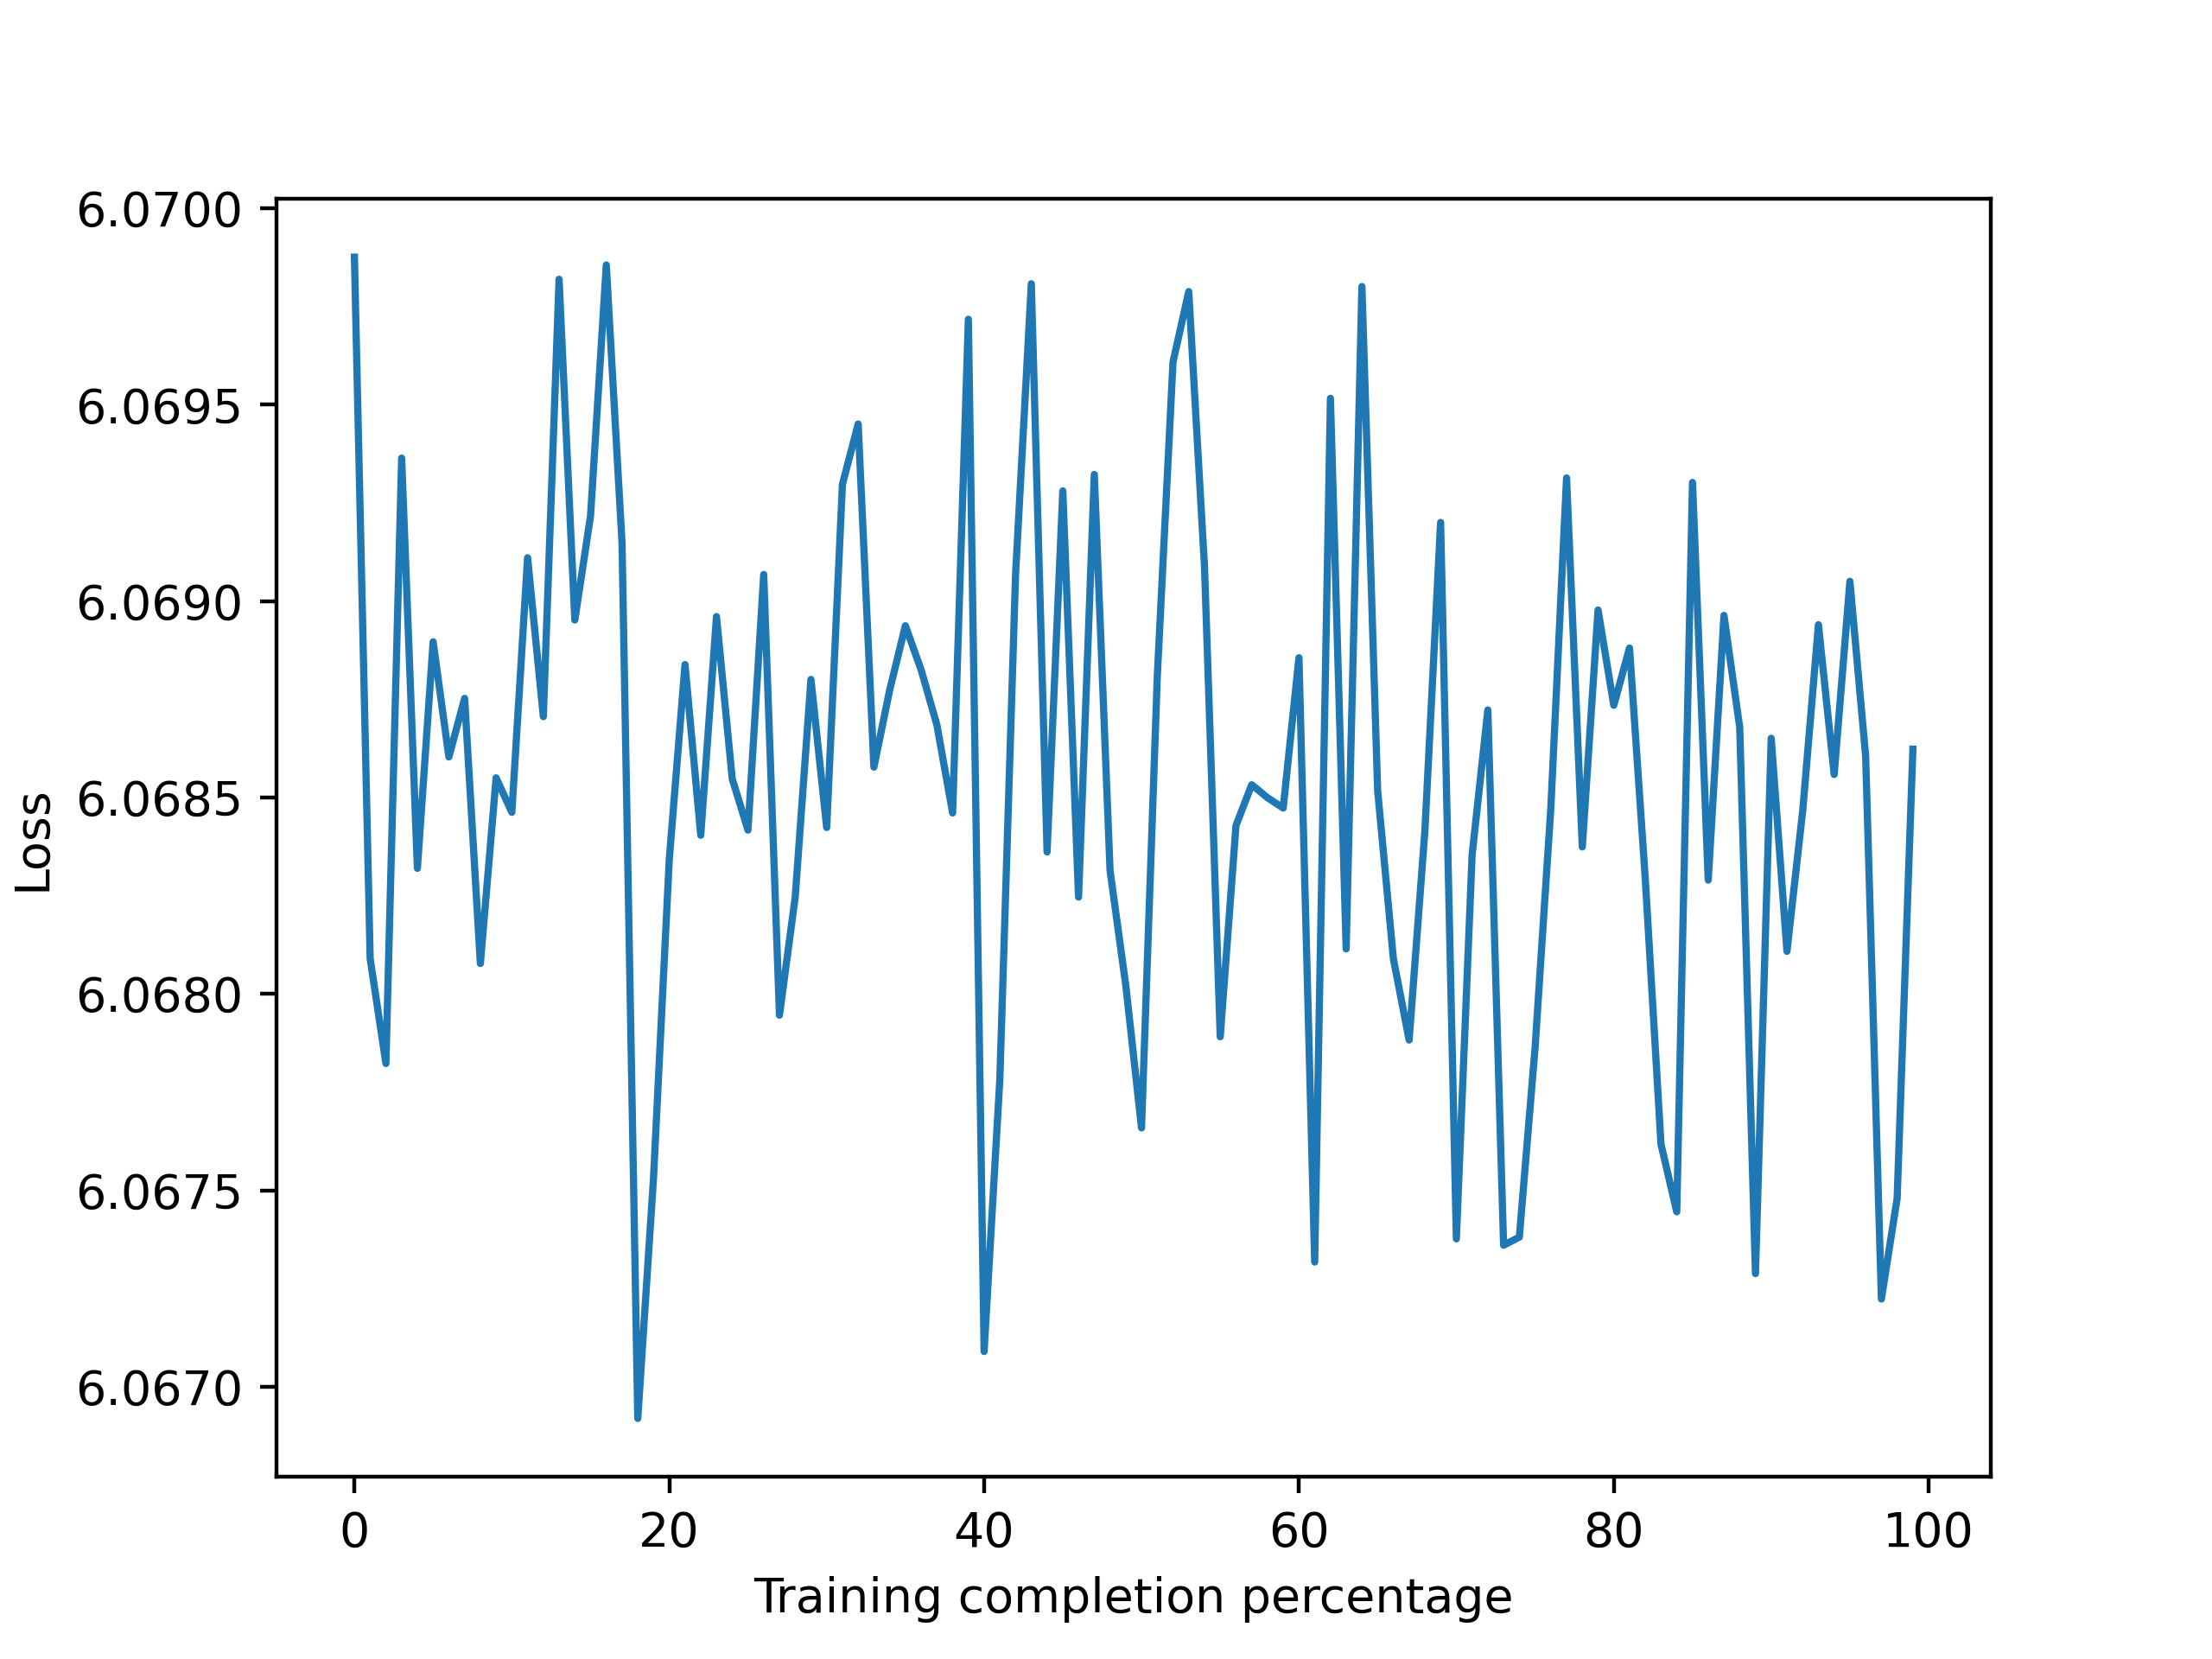
\includegraphics[scale=0.9]{loss_nograd.png}
        \caption{Loss without back propagation}
        \label{fig:nograd}
    \end{figure}
    
\end{enumerate}


\subsection{Training without updating the model parameters}
In this experiment, the \textbf{loss.backward()} method calculated the gradients. However, the model parameters were not updated by commenting the line number 16 and 17 from code listing \ref{code:train_function}. Notice in the figure \ref{fig:nograd} and figure \ref{fig:womp}, the loss is not reaching zero towards the end of the training. Indicating that in both the cases the model has not learned the product name patterns for the classification task.

\begin{figure}[H]
    \centering    
    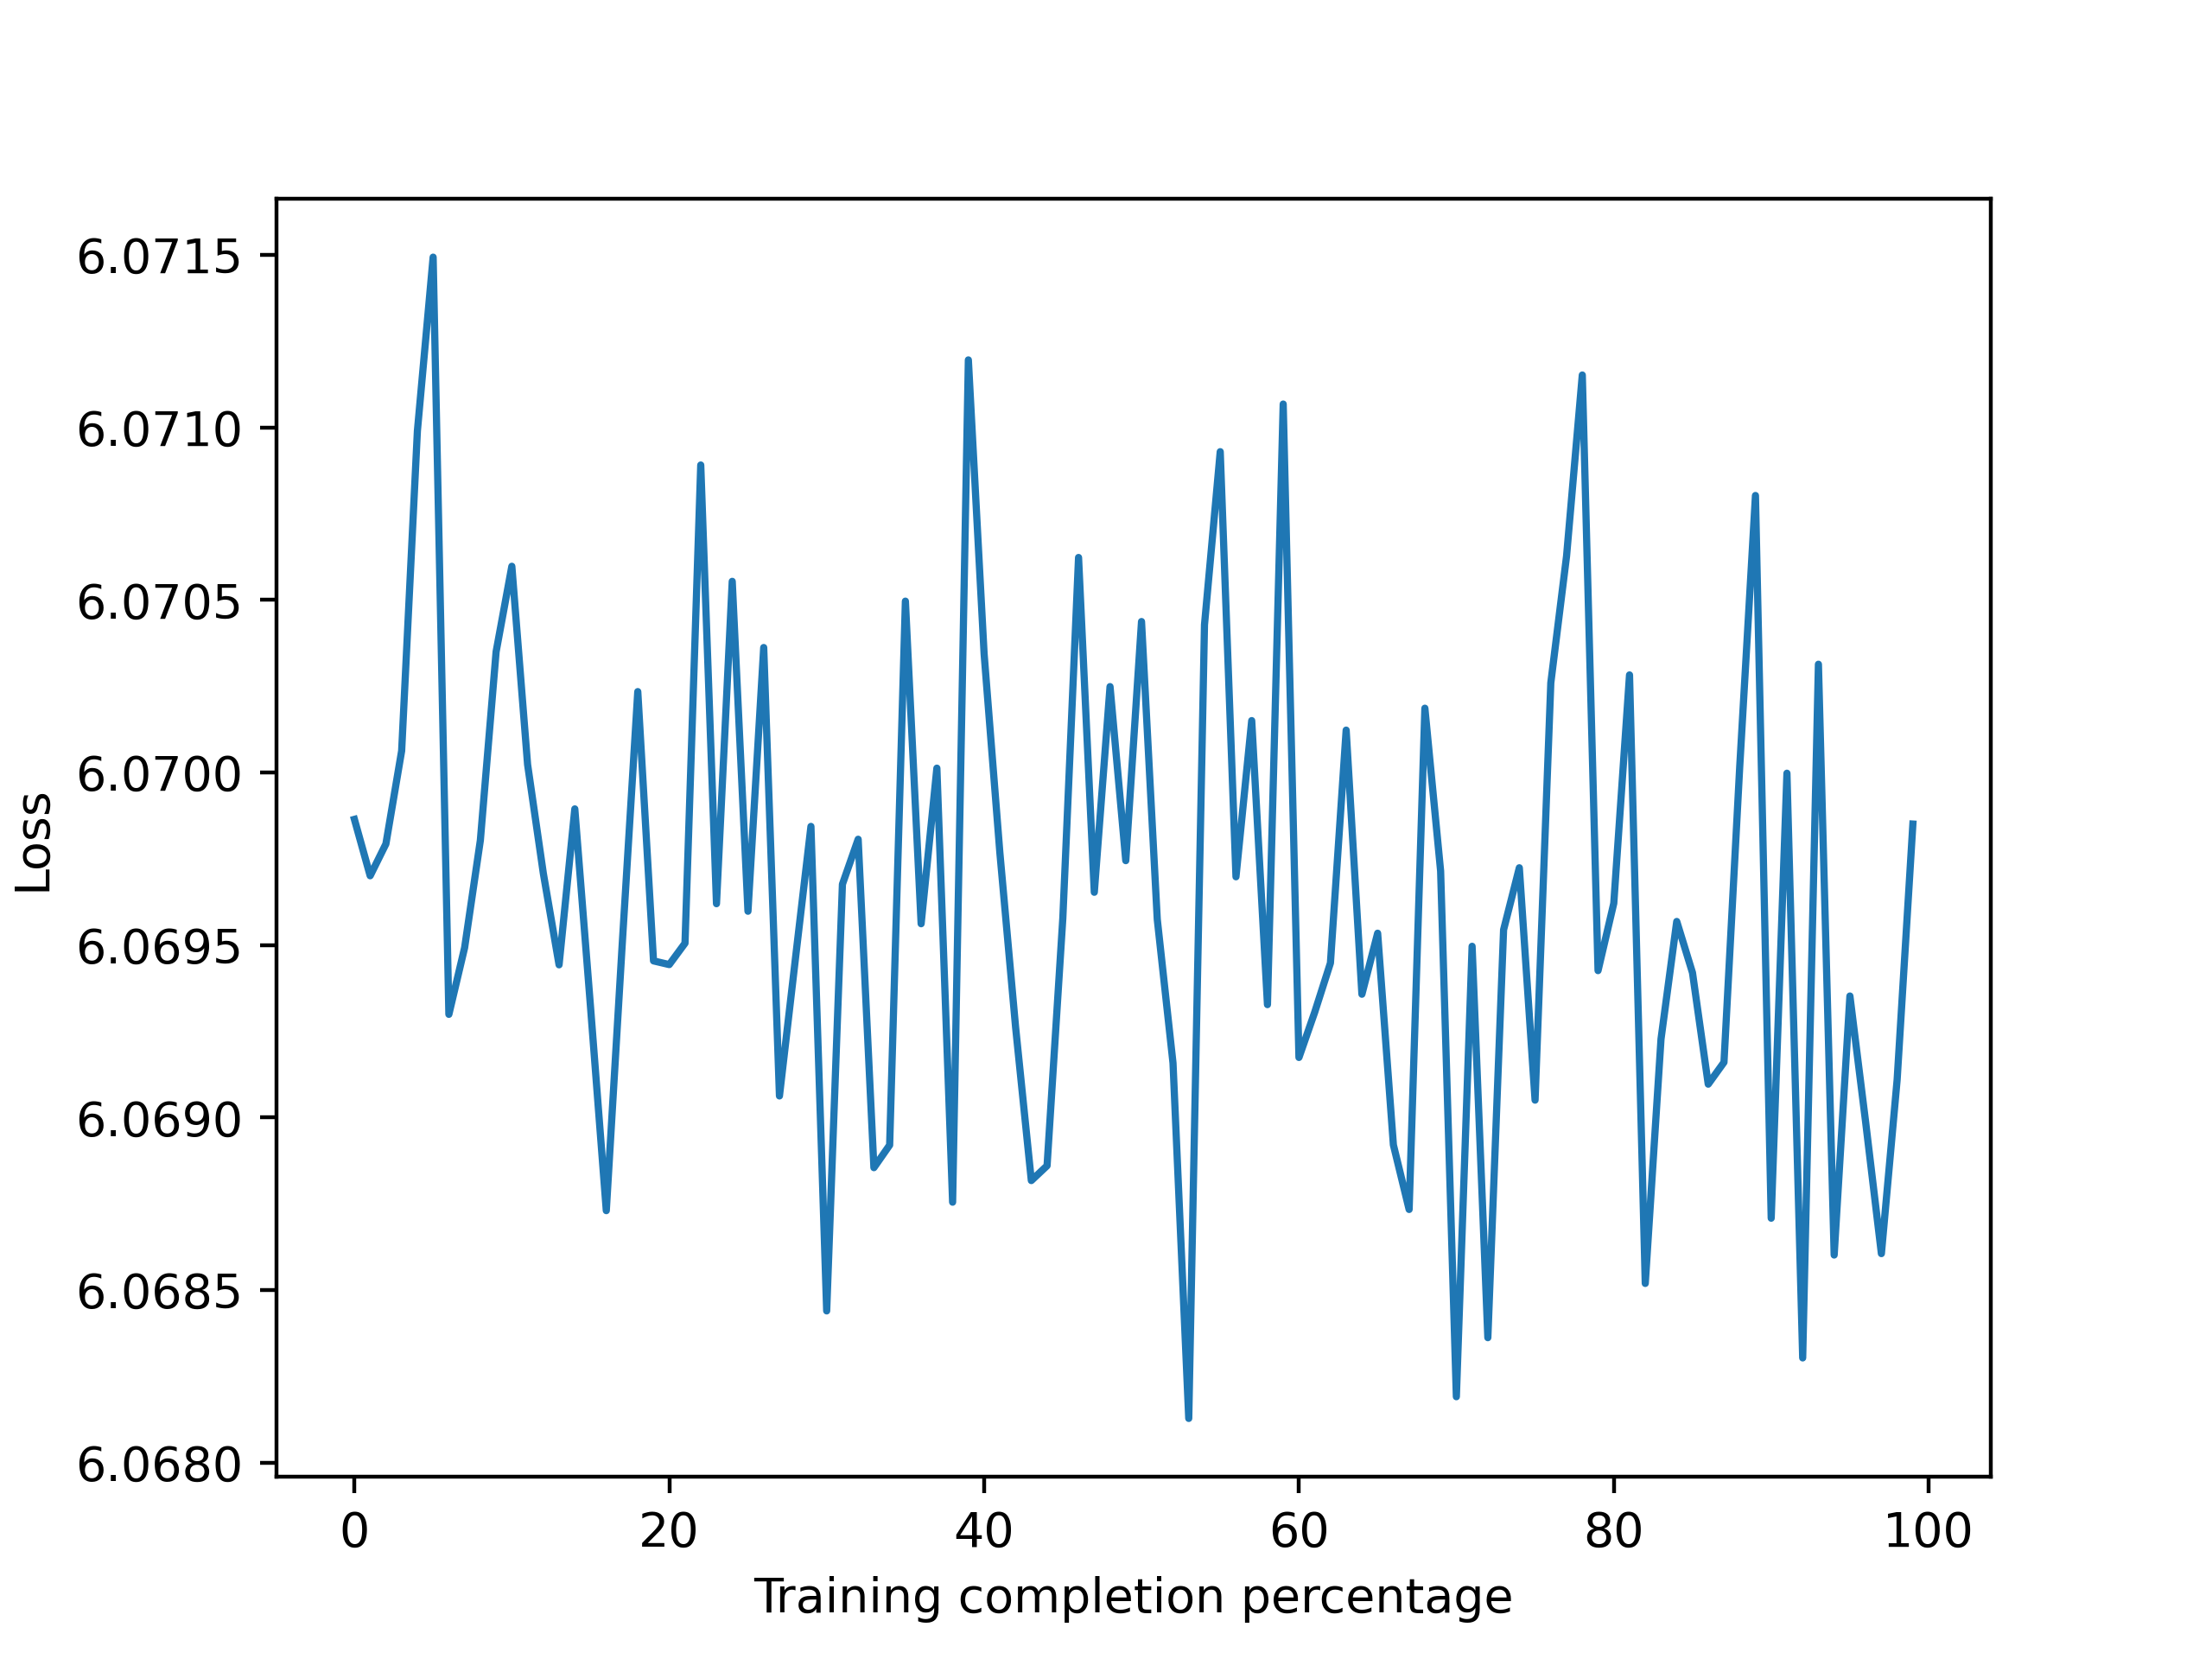
\includegraphics[scale=0.9]{loss_womp.png}
    \caption{Loss without updating the model parameters}
    \label{fig:womp}
\end{figure}

\subsection{Training with manually updating the model parameters} \label{sec:tmump}

The code listing \ref{code:mump} iterates through the parameters and updates their value based on the gradients computed during back propagation. 

\begin{lstlisting}[language=Python,caption={Manual gradient updation}, label={code:mump}]
    # Add parameters' gradients to their values, multiplied by learning rate
        for p in self.rnn.parameters():
            p.data.add_(p.grad.data, alpha=-self.learning_rate)
\end{lstlisting}

In code \ref{code:mump}, the parameter ``p.data'' is a tensor. The method  ``add\_()'' multiplies the argument and then add the product value to the tensor data ``p.data''. In this case, the negative value of ``learning\_rate'' is multiplied with the parameter gradient data and then the value is added to the ``p.data'' attribute.

\begin{figure}[H]
    \centering    
    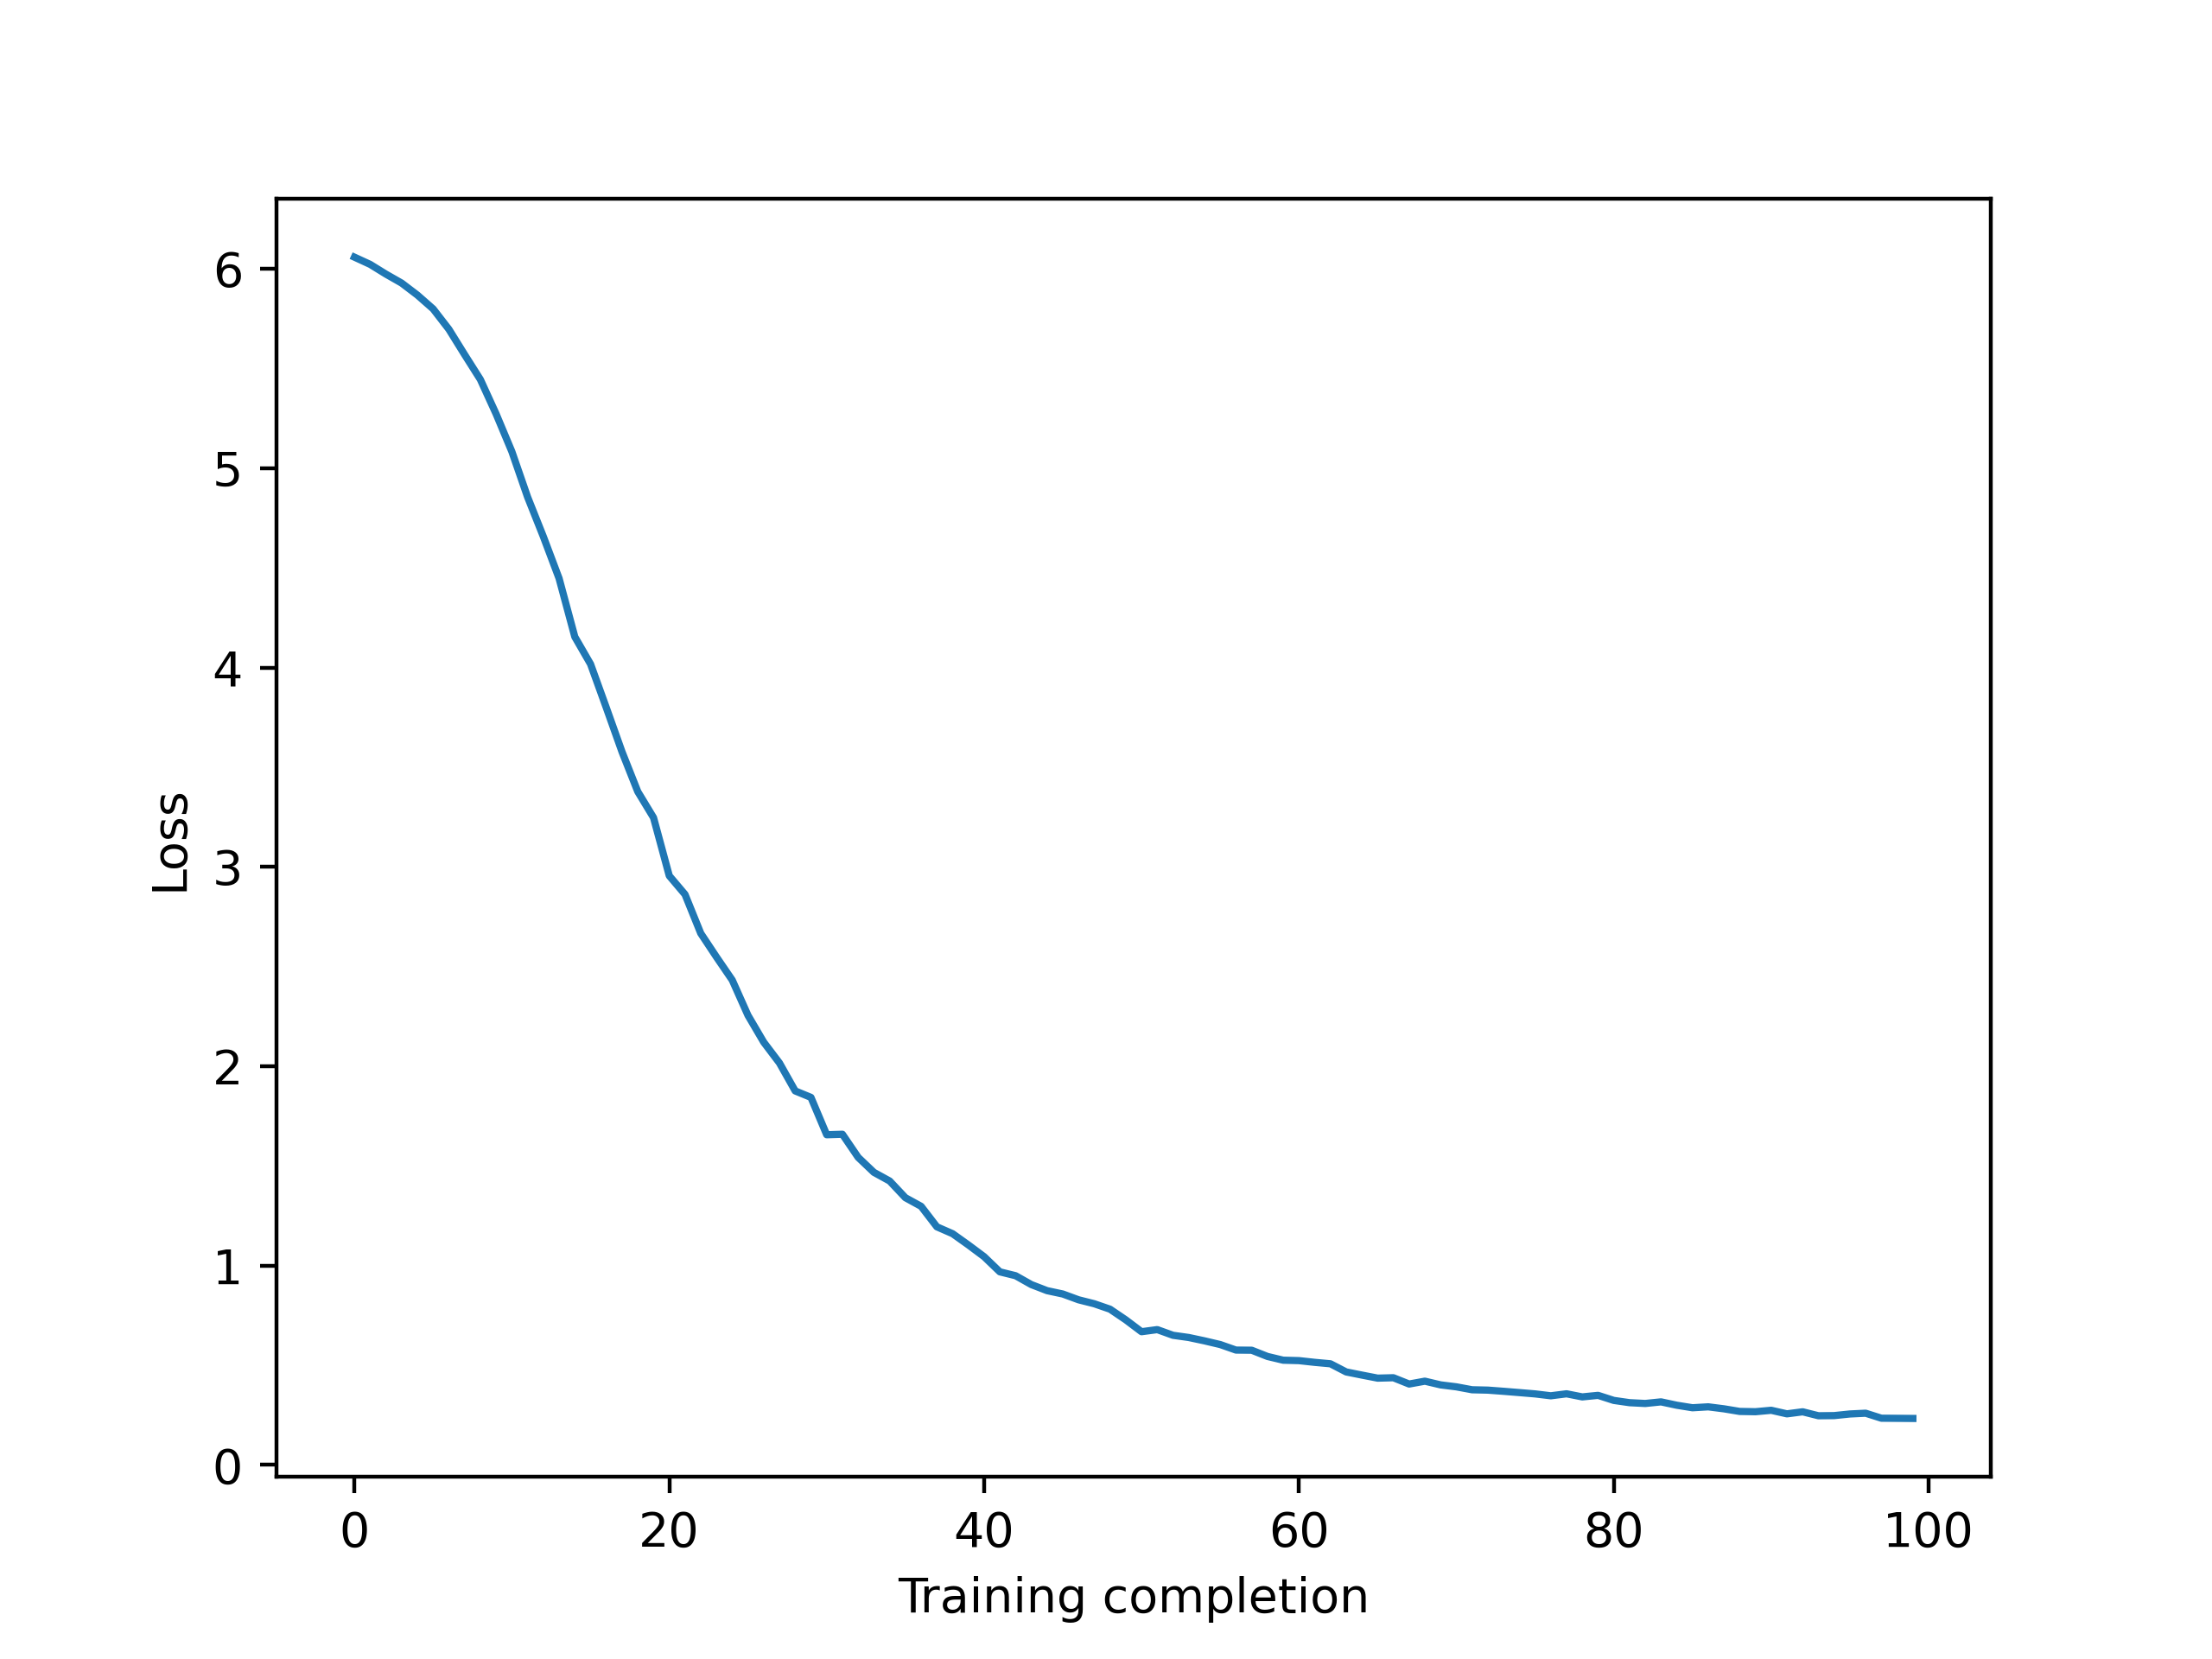
\includegraphics[scale=0.9]{loss_wmp.png}
    \caption{Loss with manually updating the model parameters with learning rate}
    \label{fig:wmp}
\end{figure}


\subsection{Updating the hidden number of units}

The model is described as a \acl{DAG} describing how functions are composed together. Consider having three functions $f(x) = f_3(f_2(f_1(x)))$ connected in a chain. $f_1$ is the first layer of the network, $f_2$ the second and so on. In the example of a classifier, $y=f_*(x)$ maps an input $ x $ to a category $ y $. The final layer of the network is called the output layer. The training data specifies what the output layer must do at each point $x$, that is to produce a value close to $y$. As the training data does not show the desired output for other layers, they are called \textbf{hidden layers}  \parencite[Chapter 3]{Goodfellow-et-al-2016}.  \parencite{zhang2021dive} describes the concept of \textbf{hidden state} which are inputs at step $t$ can only be computed with previous input at step $ t-1 $. \acf{RNN} are neural network with hidden states.

\subsubsection{Model with only one hidden state}
In this experiment, only one hidden state has been assigned to the \acs{RNN} network. As illustrated in figure \ref{fig:unihidden}, the loss reduces gradually. However, the model is yet under fit for the classification task. The loss not reaching zero towards the end of the training indicates that the model has not learned anything significant.

\begin{figure}[H]
    \centering    
    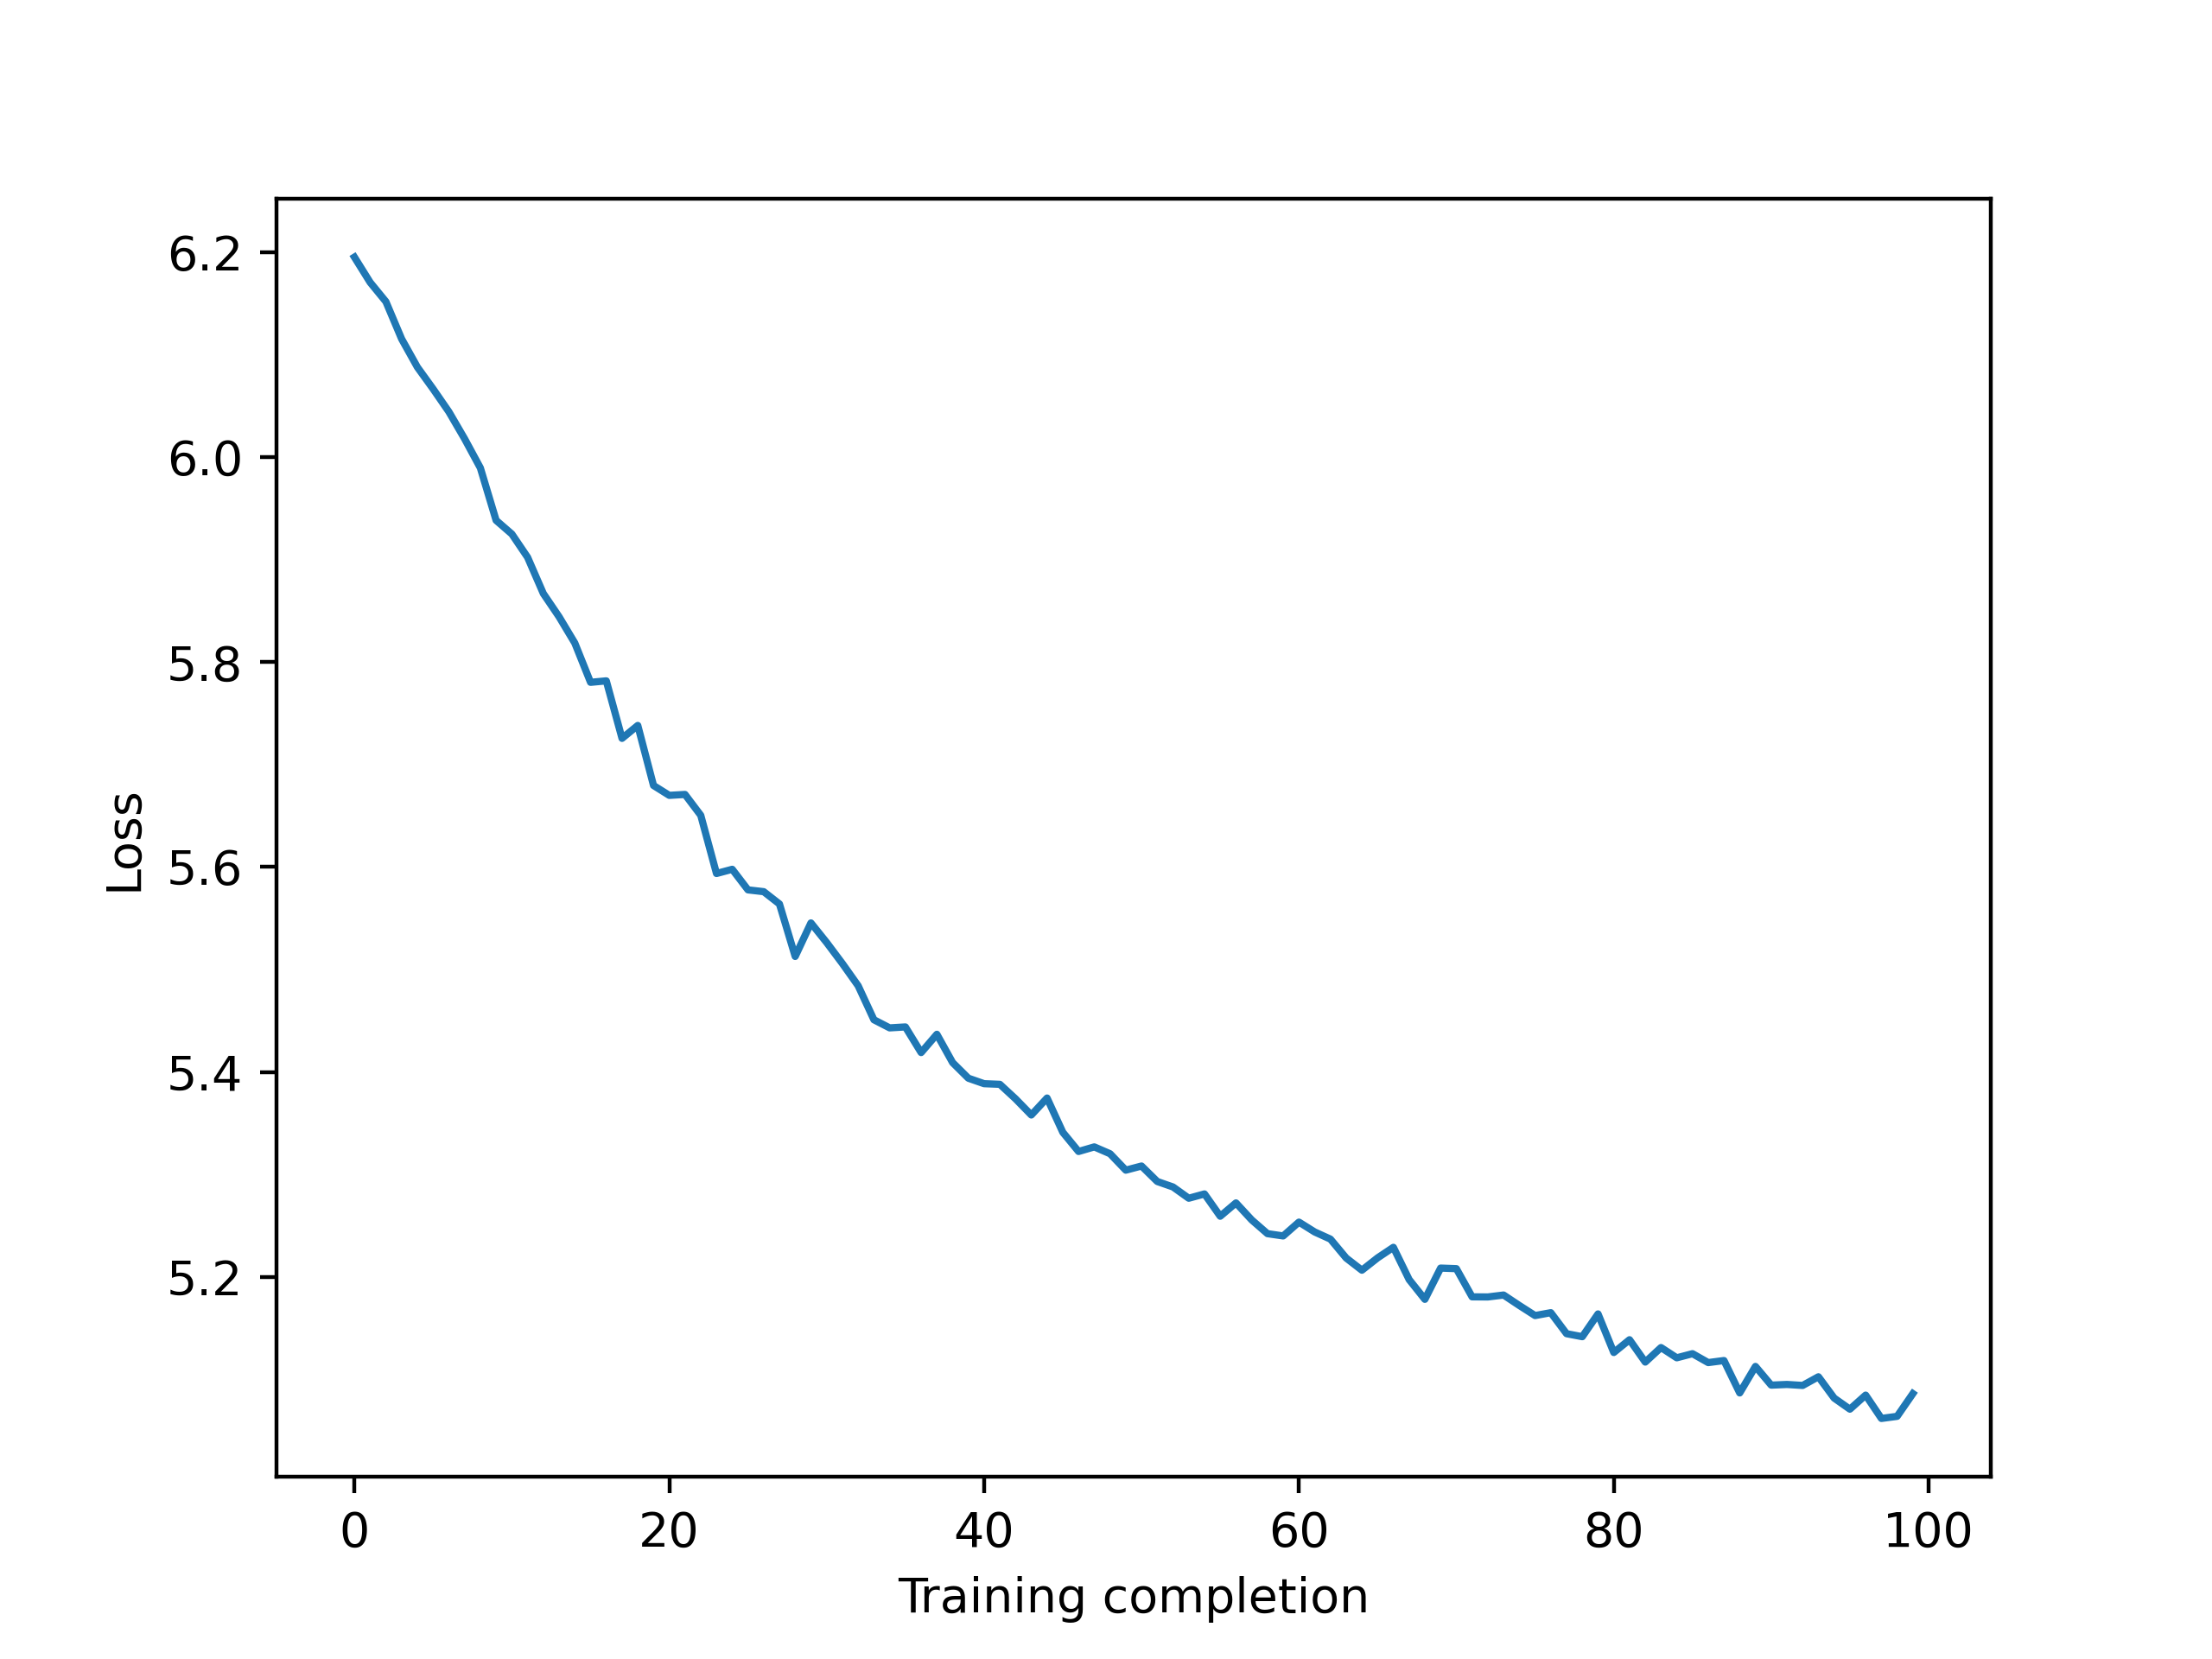
\includegraphics[scale=0.9]{loss_1hidden.png}
    \caption{Model with only one hidden state}
    \label{fig:unihidden}
\end{figure}

\subsubsection{Model with only 10 hidden state}
Increasing the number of hidden state to 10 units gave the desired result.  As seen in figure \ref{fig:10hidden}, the loss has reached near zero by end of the training. This model is able to predict the category based on the pattern of name.
\begin{figure}[H]
    \centering    
    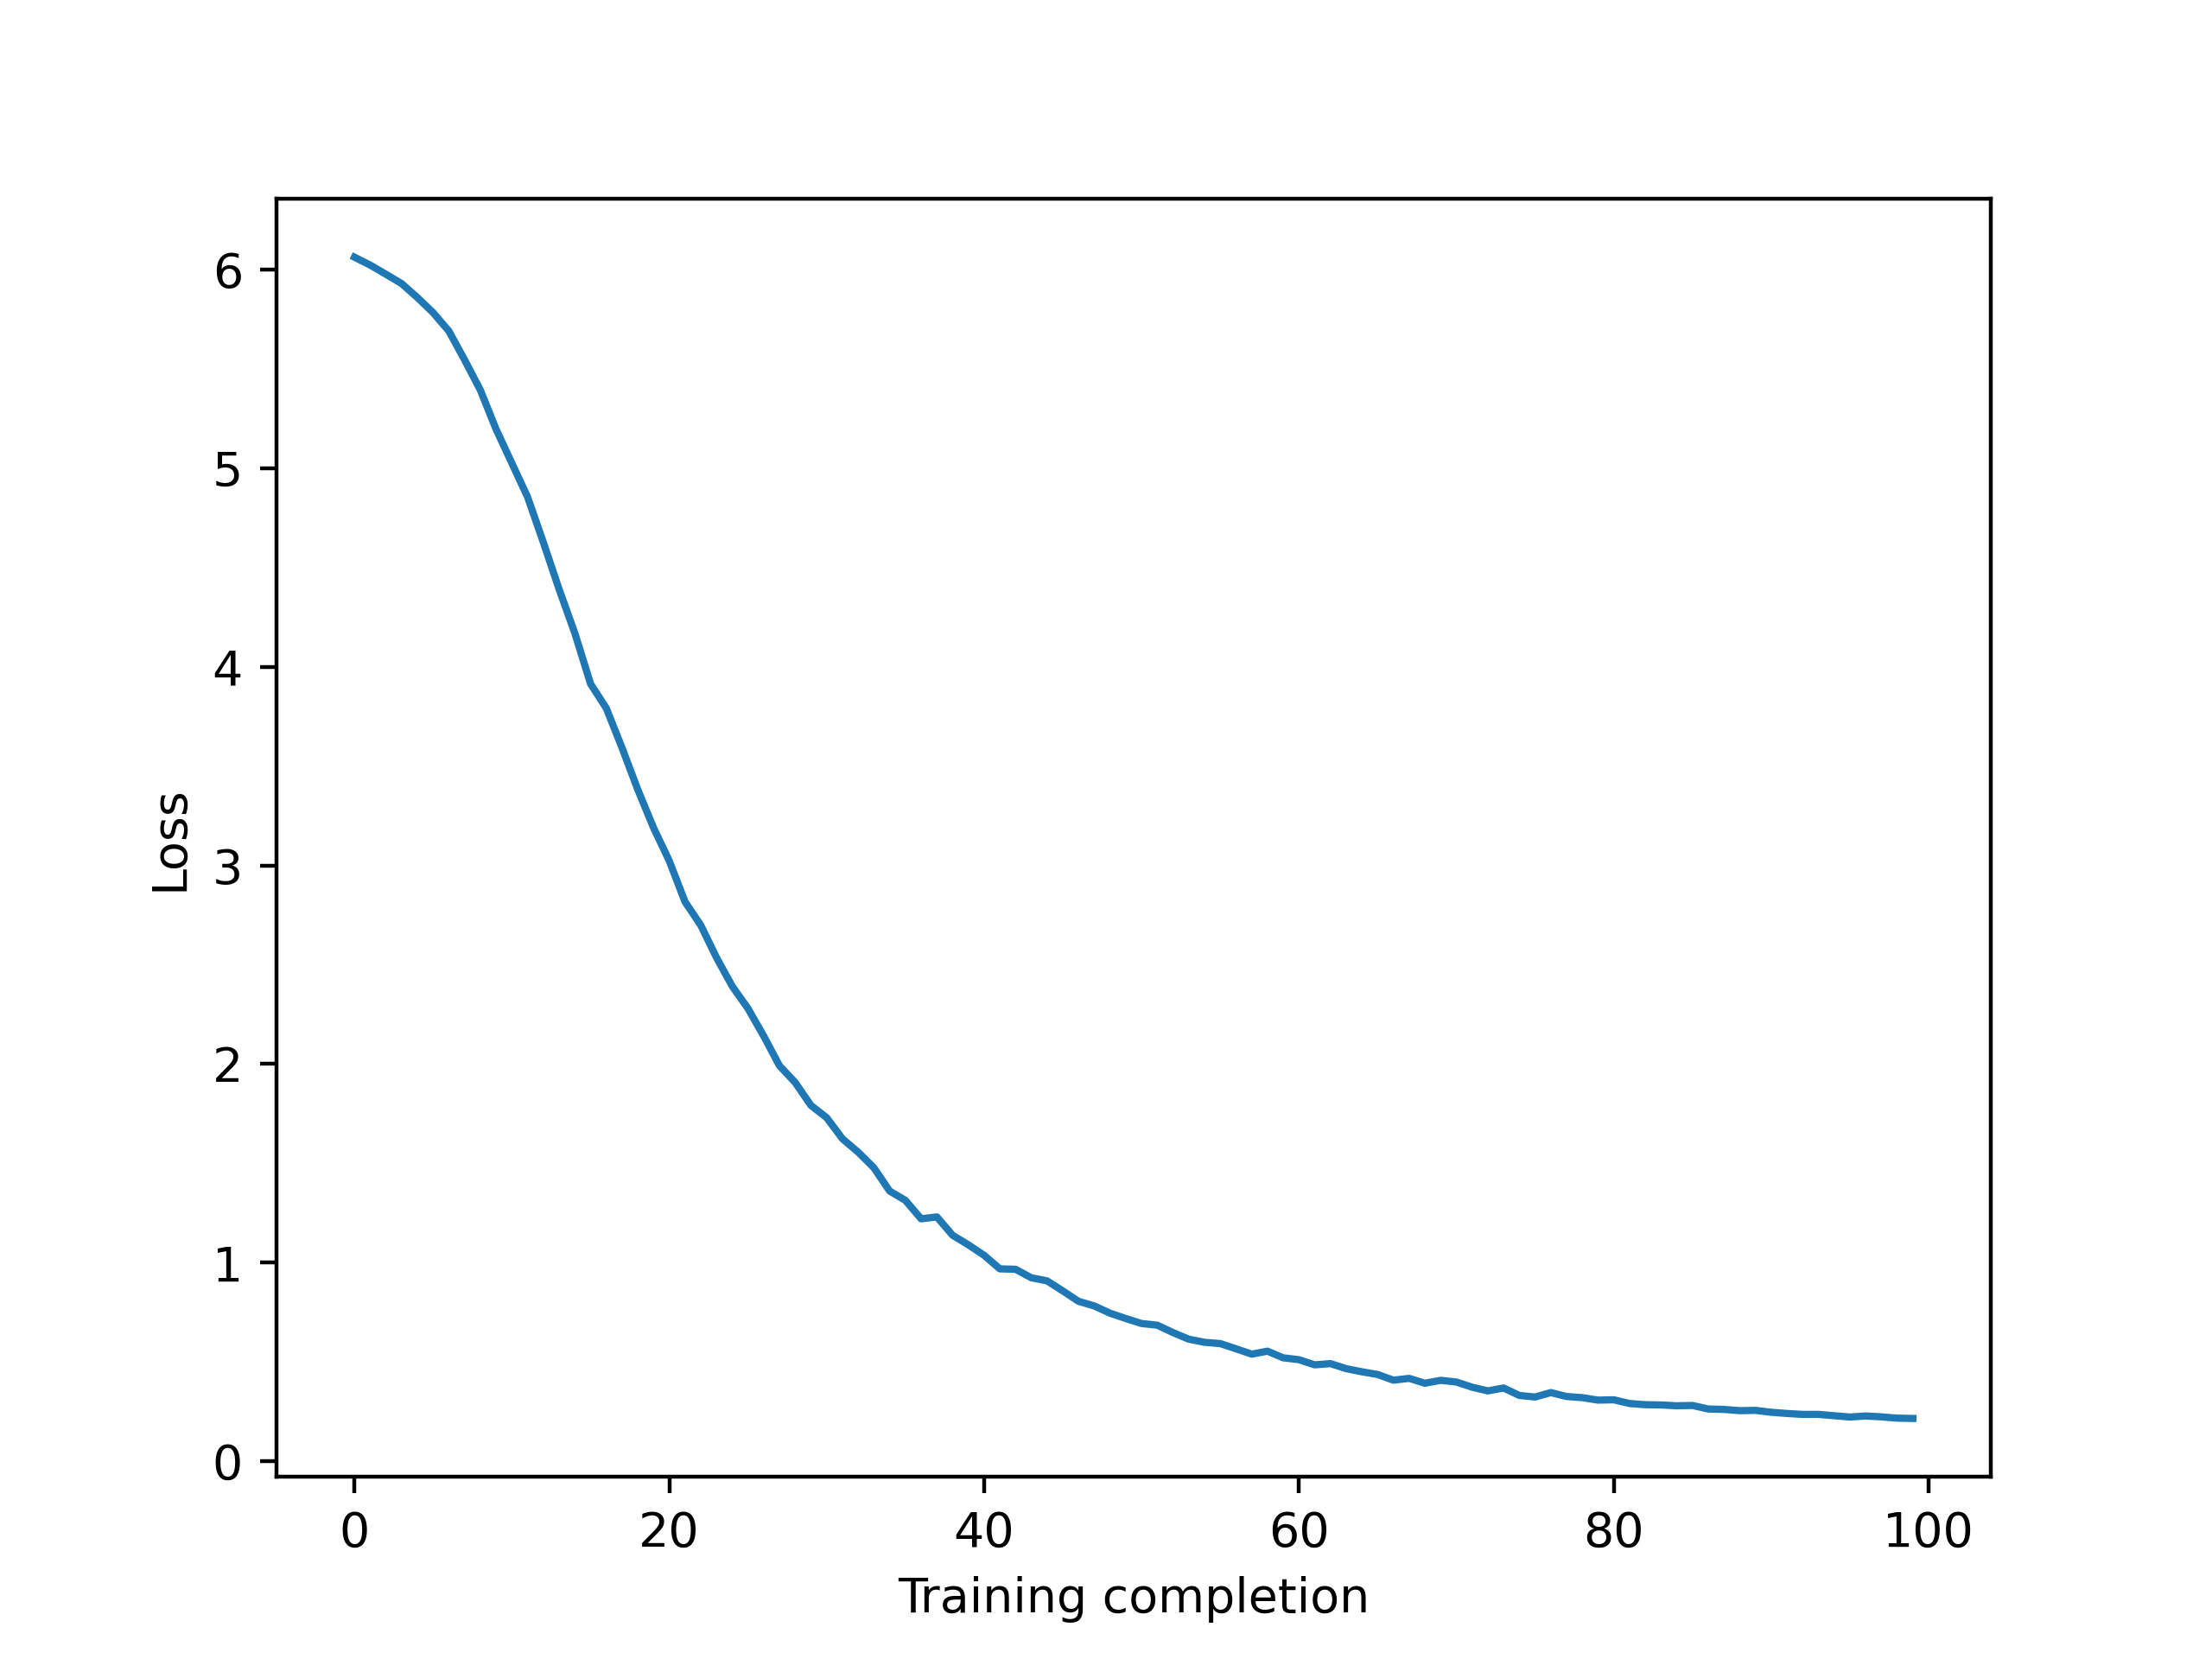
\includegraphics[scale=0.9]{loss_10h.png}
    \caption{Model with only 10 hidden state}
    \label{fig:10hidden}
\end{figure}

\subsection{Gradient decent step adjustment}

As stated in section \ref{sec:backward}, the method \textbf{loss.backward()} computes the gradients by applying chain rule of calculus for each function $f(x)$. The derivative of this function is denoted as $f'(x)$ \\ or as $\frac{dy}{dx}$. $f(x)$ can be reduced by moving $x$ in small with steps opposite sign of derivative is called gradient decent \parencite{cauchy}.  \parencite[section 4.3]{Goodfellow-et-al-2016} presents an equation \ref{eq:update_rule}.

\begin{align}
    x_i = x_i - \epsilon \frac{\partial}{\partial x_i} f(x) \label{eq:update_rule}
\end{align}

\begin{itemize}
    \item \( x_i \): The \(i\)th parameter of the model (weight or coefficient).
    \item \( \epsilon \): The learning rate, a positive scalar which determines the size of the step.
    \item \( f(x) \): The cost or loss function trying to minimize.
    \item \( \frac{\partial}{\partial x_i} f(x)\): The partial derivative  measures how \( f \) changes as only the variable \( x_i \) increases at point  \( x \).
\end{itemize}


In section \ref{sec:tmump}, refer to the code listing \ref{code:mump}, based on the equation \ref{eq:update_rule} we conclude that the variable \textit{p.grad.data} represents the partial derivative \( \frac{\partial}{\partial x_i} f(x) \) and the negative value of variable \textit{self.learninig\_rate} is included to subtract product of  variable \textit{p.grad.data} and variable \\ \textit{self.learninig\_rate} with variable \textit{p.data}. The same result can be achived by using pytorch's  \textit{subtract\_} method without negating the value of \textit{self.learninig\_rate}.

\begin{lstlisting}[language=Python,caption={Manual gradient updation with substract\_}, label={code:mumps}]
    # Add parameters' gradients to their values, multiplied by learning rate
        for p in self.rnn.parameters():
            p.data.subtract_(p.grad.data, alpha=self.learning_rate)
\end{lstlisting}

\section{\acf{CLR}}

Learning rate is an important parameter to tune the training of deep neural network. \parencite{Smith.03062015} describes a new method to set the learning rate called \acf{CLR}. In this method the learning rate in the training cyclically vary between the reasonable boundaries of the learning rate instead of having a fixed learning rate.

The steps involved in training a model with \acs{CLR} are as follows :

\begin{enumerate}
    \item Define the Learning rate range or reasonable boundary value: \\
    In this step, by linearly increasing the learning rate during training can specify the learning rate range in which an optimal accuracy is obtained. The lower point of range can be referred as $base\_lr$ and higher point as $max\_lr$.
    \item Training the model by gradually decreasing the learning rate to $base\_lr$ and again increasing the learning rate to $max\_lr$ over an interval of a constant step size.
\end{enumerate}


\subsection{Learning rate range}

\begin{enumerate}
    \item Experiment by setting $base\_lr$ and $max\_lr$  manually : \\
    In this experiment, the learning rate range is set manually to very low and high values. Numpy np.linspace() \parencite{harris2020array} returns the evenly spaced numbers between the  $base\_lr$ and $max\_lr$ over a specified interval.

    The result of training process the model with $base\_lr =1 \times 10^{-11}$ and $max\_lr=0.9$.\\
    In figure \ref{fig:Loss value} notice that at 32 \% of training completion with learning rate $\approx$ 0.2 the loss started to explode. Hence, we conclude that the  $max\_lr < 0.2$

    \begin{figure}[H]
        \centering    
        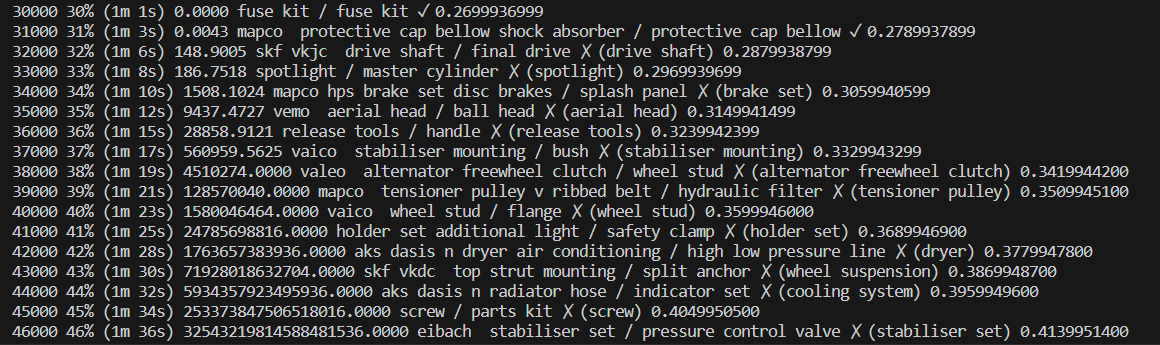
\includegraphics[scale=0.7]{loss_nan.png}
        \caption{Result: Loss value returning nan}
        \label{fig:Loss value}
    \end{figure}


    \item In the next experiment, we set the $max\_lr = 0.2$. \\
    The classification model successfully completed the training and was able to predict the category.
    \begin{figure}[H]
        \centering    
        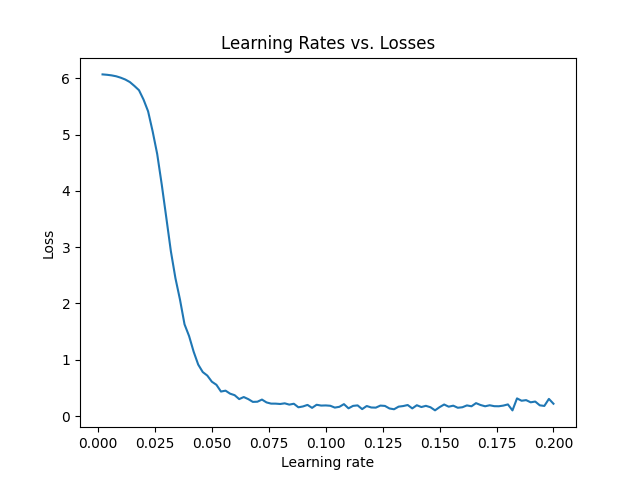
\includegraphics[scale=0.9]{loss_lr_02.png}
        \caption{Loss vs Learning rate; where $max\_lr = 0.2$}
        \label{fig:Loss value at 0.2}
    \end{figure}
    
    As illustrated in figure \ref{fig:Loss value at 0.2}, in the graph plotted of Loss Vs Learning rate. The model started to learn at learning rate $\epsilon = 0.04$ onwards. We will further reduce the $max\_lr$.

\end{enumerate}